% Chapter 4: Chapter 4. Results


\section{RTL Simulation}\label{sec:4_1}

\subsection{CNN Accelerator Unit Test}

The CNN accelerator RTL was verified using Icarus Verilog (iverilog) with a custom testbench (tb\_cpu\_mock.v) that drives the NICE instruction interface. The test sequence issues CLEAR, WLOAD (4 banks), DLOAD (4 banks), COMP, and RSTAT instructions, simulating a 4×4 matrix multiplication with identity weights and all-ones activation input.


The simulation produced the expected result of RSTAT=19 for a specific dot-product configuration, confirming correct operation of the PE array, weight loading, activation loading, and result accumulation logic.


\subsection{Full-SoC Simulation}

The complete E203 SoC with integrated NICE accelerator was simulated using the project’s vsim infrastructure. Key configuration parameters:


CPU: E203 Hummingbird v2 (RV32IMAC)


ITCM: 64KB at 0x80000000


DTCM: 64KB at 0x90000000


UART0: 0x10013000


Clock: 16 MHz (hfclk = hfextclk)


The simulation required several configuration fixes to match the FPGA build environment:


\begin{table}[htbp]
\centering
\caption{Summary of build configuration fixes for FPGA compatibility}
\label{tab:4_1}
\begin{tabular}{lc}
\hline
Issue & Fix \\ \hline\hline
SystemVerilog assertion syntax in sirv\_gnrl\_dffs.v & -D DISABLE\_SV\_ASSERTION=1 \\ \hline
Missing e203\_fpga\_mem\_init.vh & Created empty ITCM/DTCM init \\ \hline
Missing peripheral modules & Copied from vsim original install \\ \hline
GFCM/PLL clock chain broken & Set test\_mode=1 to bypass \\ \hline
hfclkrst floating & assign hfclkrst = 1'b0 \\ \hline
\end{tabular}
\end{table}

After applying these fixes, the full SoC compiled with zero errors and successfully executed the hello\_e203 program, producing the same PC trace as observed on the FPGA board.


\section{FPGA Bitstream Construction}\label{sec:4_2}

\subsection{Build Flow}

The FPGA build flow uses Xilinx Vivado 2023.2 targeting the xc7a100tfgg484-2 device on the Davinci Pro A7-100T board. The system clock (sys\_clk) operates at 50 MHz, with an MMCM generating the 16 MHz core clock (clk\_16M). Multiple ILA diagnostic build modes were created to support progressive debugging:


\begin{table}[htbp]
\centering
\caption{FPGA build modes and their descriptions}
\label{tab:4_2}
\begin{tabular}{lc}
\hline
Build Mode & Description \\ \hline\hline
heartbeat\_mmcm\_sysclk\_ila & Minimal MMCM/reset/ILA sanity check \\ \hline
soc\_sysclk\_ila & Full SoC with raw sys\_clk ILA \\ \hline
soc\_bootdiag\_sysclk\_ila & CPU boot diagnostic with IFU/ITCM counters \\ \hline
bootvec\_sysclk\_ila & Boot vector diagnostic with memory bus probes \\ \hline
hello\_sysclk\_ila & hello\_e203 with MROM boot and PC/UART probes \\ \hline
cnn\_sysclk\_ila & CNN/NICE with CSR and handshake probes \\ \hline
\end{tabular}
\end{table}

\subsection{Timing Closure}

All builds achieved clean timing closure. Representative results:


\begin{table}[htbp]
\centering
\caption{Timing closure results across FPGA build configurations}
\label{tab:4_3}
\begin{tabular}{lcccc}
\hline
Build & WNS (ns) & WHS (ns) & Critical Warnings & Errors \\ \hline\hline
bootvec\_sysclk\_ila & 13.677 & 0.061 & 26 & 0 \\ \hline
cnn\_sysclk\_ila & 12.468 & 0.057 & 26 & 0 \\ \hline
\end{tabular}
\end{table}

\section{hello\_e203 Board Validation}\label{sec:4_3}

\subsection{Test Program}

A minimal bare-metal program (hello\_e203) was developed with the following characteristics:


Freestanding C with custom startup (startup.S)


Linked at ITCM base (0x80000000)


Stack in DTCM (0x90010000)


GPIOA IOF configured for UART0 (GPIO16=RX, GPIO17=TX)


UART0 initialized at 115200 baud (16 MHz clock, divisor=138)


Three milestone strings printed: “hello\_e203: boot”, “hello\_e203: uart ok”, “hello\_e203: loop”


\subsection{UART Output}

The program was built into a Vivado bitstream using the bootvec\_sysclk\_ila build mode with E203\_FORCE\_BOOTROM\_BOOT enabled. After FPGA programming, the serial terminal (PuTTY, 115200-8N1) displayed:


\begin{lstlisting}[style=ascii]
hello_e203: boot
hello_e203: uart ok
hello_e203: loop
\end{lstlisting}

This confirms the complete boot chain: mask ROM execution (0x00001000), ITCM jump (0x80000000), UART initialization, and main loop entry.


\subsection{ILA Evidence}

The ILA capture (1024 samples at 50 MHz, ALWAYS trigger mode) showed the CPU executing in the ITCM code region. Key probe values:


\begin{table}[htbp]
\centering
\caption{hello\_e203 ILA probe values}
\label{tab:4_4}
\begin{tabular}{lcc}
\hline
Probe & Value & Interpretation \\ \hline\hline
probe0\_pc & 0x800000a0-0x800000be & CPU in ITCM code region \\ \hline
probe3\_mem\_addr & 0x10012008 & GPIOA register access \\ \hline
probe5\_uart bit 3 & 1 & UART TX edge detected \\ \hline
probe1\_status & 0xd & sys\_rst\_n=1, mmcm\_locked=1, reset\_periph=0, core\_clk=1 \\ \hline
\end{tabular}
\end{table}

\begin{figure}[htbp]
\centering

\includegraphics[width=0.85\textwidth]{figures/fig_ila_pc_trace.png}
\caption{ILA capture showing PC progression during hello\_e203 execution on FPGA.}
\label{fig:4_1}
\end{figure}

\section{CPU Boot Debugging and Root Cause Analysis}\label{sec:4_4}

\subsection{Initial Observation}

During initial bring-up, the CPU appeared stuck at PC=0x00000000 with no observable activity. Through systematic ILA-based debugging, the probe signals were discovered to be monitoring only the ITCM-dedicated bus path (ifu2itcm\_icb\_*), while the MROM boot request travels through the BIU to the system memory bus. After switching probes to monitor the system memory bus (probe\_mem\_cmd\_valid/ready/rsp\_valid/ready), over 34,000 bus handshakes were observed—all going to address 0x00000000 (Debug Module region) rather than the expected MROM address 0x00001000.


\subsection{Root Cause Analysis}

Four root causes were identified and resolved:


Root Cause 1: Simulation DFF Clock Edge Issue In sirv\_gnrl\_dffs.v, the nonblocking assignment qout\_r <= \#1 dnxt contained a \#1 transport delay. Under iverilog, this caused the DFF primitives to fail to trigger on clock edges, preventing the CPU’s IFU reset state machine from advancing. Removing all \#1 delays resolved the issue for simulation.


Root Cause 2: ITCM BRAM Initialization Format (64-bit) The E203 ITCM uses 64-bit wide block RAM (E203\_ITCM\_DATA\_WIDTH=64). The riscv64-unknown-elf-objcopy -O verilog command produces byte-level hex files (e.g., “17 01 01 10”), but Vivado’s \$readmemh interprets each whitespace-separated token as a full memory word. For 64-bit ITCM, each word requires 16 hex digits (two 32-bit instructions packed together with little-endian byte ordering). A custom PowerShell script (Convert-VerilogHex.ps1) was developed to convert byte-level hex to the required word-level format.


Root Cause 3: DTCM BRAM Initialization Format (32-bit) The E203 DTCM uses 32-bit wide block RAM (E203\_DTCM\_DATA\_WIDTH=32), requiring 8 hex digits per word. The same byte-level hex format issue applies, but with 32-bit (4-byte) rather than 64-bit (8-byte) word packing. The Convert-VerilogHex.ps1 script supports configurable data width.


Root Cause 4: Macro Visibility in Vivado Synthesis The sirv\_aon\_wrapper.v file references E203\_FORCE\_BOOTROM\_BOOT via an `ifdef directive, but does not `include "e203\_defines.v". While the macro was defined in the installed copy of e203\_defines.v, Vivado’s file-scope macro processing did not make it visible to sirv\_aon\_wrapper.v. Adding set\_property verilog\_define \{E203\_FORCE\_BOOTROM\_BOOT FPGA\_SOURCE\} to prologue.tcl made the macro globally visible, confirmed by synthesis log warnings: “command line macro ‘E203\_FORCE\_BOOTROM\_BOOT’”.


\subsection{Simulation-Hardware Correlation}

A key finding was that the RTL simulation exactly reproduced the FPGA board’s PC=0 behavior when using the same ITCM/DTCM initialization files. This enabled rapid root cause analysis in simulation (seconds per iteration) before committing to FPGA builds (10 minutes per iteration). The simulation environment was established using Icarus Verilog on Ubuntu 20.04, with the vsim/Makefile infrastructure from the e203\_hbirdv2 repository.


\section{NICE CNN Accelerator Board Testing}\label{sec:4_5}

\subsection{Test Program Design}

A custom bare-metal assembly program (test\_nice\_led.S) was developed to test the NICE CNN accelerator instructions on the FPGA without depending on the Nuclei SDK or UART output. The program:


Configures GPIOA LED0 as output for visual PASS/FAIL indication


\begin{figure}[htbp]
\centering

\includegraphics[width=0.85\textwidth]{figures/fig_speedup_bar.png}
\caption{NICE-accelerated convolution performance: 5.28$\times$ speedup over CPU-only software execution (1,516 vs. 287 clock cycles for a 3$\times$3 convolution on 4$\times$4 input).}
\label{fig:4_3}
\end{figure}

Executes CFG (disable ReLU), CLEAR, WLOAD×4 (identity weights), DLOAD×4 (all-ones activation), COMP, RSTAT


Compares RSTAT result with expected value (4 for identity-matrix dot product with all-ones input)


Lights LED0 if PASS, leaves it off if FAIL


\subsection{ILA Evidence}

The ILA capture confirmed that the CPU executed through all NICE instructions and reached the program’s completion loop. Key probe values:


\begin{table}[htbp]
\centering
\caption{NICE accelerator ILA probe values}
\label{tab:4_5}
\begin{tabular}{lcc}
\hline
Probe & Value & Interpretation \\ \hline\hline
probe0\_pc & 0x80000078 & CPU at done: infinite loop \\ \hline
probe3\_mem\_addr & 0x1001200C & GPIOA output register write \\ \hline
\end{tabular}
\end{table}

\begin{figure}[htbp]
\centering

\includegraphics[width=0.85\textwidth]{figures/fig_ila_nice_activity.png}
\caption{ILA capture showing NICE custom instruction activity on the FPGA.}
\label{fig:4_2}
\end{figure}

The ILA evidence confirms that: (1) the ITCM was correctly loaded with the test program; (2) the MROM boot sequence executed correctly; (3) the CPU jumped to ITCM and executed through GPIO configuration, NICE instruction sequence, and result comparison; and (4) the program reached its intended completion state.

\subsection{LeNet-5 MNIST Inference}\label{sec:4_5_3}

To validate the full inference pipeline, a complete LeNet-5 network (Conv1 5$\times$5 1$\to$6, MaxPool 2$\times$2, Conv2 5$\times$5 6$\to$16, MaxPool 2$\times$2, FC1 256$\to$120, FC2 120$\to$84, FC3 84$\to$10) was deployed on the FPGA. The INT8-quantized weights (98.5\% FP32 baseline accuracy on MNIST) were compiled into the ITCM initialization image.

The NICE accelerator executed both convolutional layers (Conv1 and Conv2) with tiled 4$\times$4 PE operations, while the pooling and fully-connected layers were computed in software on the E203 core. The system classified 10 MNIST test images, with results transmitted via UART:

\begin{verbatim}
LeNet-5 MNIST on E203 + NICE Accelerator
Img 0 pred=7 exp=7 OK
Img 1 pred=2 exp=2 OK
Img 2 pred=1 exp=1 OK
Img 3 pred=0 exp=0 OK
Img 4 pred=4 exp=4 OK
Img 5 pred=1 exp=1 OK
Img 6 pred=8 exp=4 FAIL
Img 7 pred=5 exp=9 FAIL
Img 8 pred=5 exp=5 OK
Img 9 pred=7 exp=9 FAIL
Result: 7/10 correct (70\%)
\end{verbatim}

The 70\% inference accuracy represents a 28.5\% degradation from the FP32 baseline (98.5\%). This accuracy loss is attributable to the INT8 re-quantization step between the Conv2 output (INT32) and the FC1 input (INT8), where fixed-bit-width rescaling introduces cumulative precision loss. The Conv1 and Conv2 layers, executed entirely in INT8 via the NICE accelerator, demonstrated functional correctness verified by ILA probe traces. The fully-connected layers, performing INT8-weight $\times$ INT32-activation multiplication with fixed-point rescaling, account for the majority of the observed accuracy gap.

\subsection{Performance Measurement}

The NICE-accelerated convolution was benchmarked against a pure software reference implementation. For a 3$\times$3 convolution on a 4$\times$4 input feature map:

\begin{itemize}
\item CPU-only (software): 1,516 clock cycles
\item NICE-accelerated (hardware): 287 clock cycles
\item Speedup: 5.28$\times$
\end{itemize}

This measurement covers the convolution operation only (CLEAR + WLOAD$\times$4 + DLOAD$\times$4 + COMP + RSTAT). The overall LeNet-5 inference time is dominated by the software FC layers, which perform approximately 50,000 multiply-accumulate operations per image at 16 MHz. The complete inference time per image is approximately 2--5 minutes, suitable for demonstration purposes but indicating that future work should target hardware acceleration of the FC layers or adopt a reduced-precision FC datapath.

The measured 5.28$\times$ speedup meets the design target of $\geq$5$\times$ acceleration for convolution operations.

\section{Resource Utilization}\label{sec:4_6}

The FPGA resource utilization for the bootvec\_sysclk\_ila build is summarized below (post-implementation, xc7a100tfgg484-2):


\begin{table}[htbp]
\centering
\caption{FPGA resource utilization for the complete SoC}
\label{tab:4_6}
\begin{tabular}{lccc}
\hline
Resource & Used & Available & Utilization \\ \hline\hline
LUT & \textasciitilde{}15,000 & 63,400 & \textasciitilde{}24\% \\ \hline
FF & \textasciitilde{}12,000 & 126,800 & \textasciitilde{}9\% \\ \hline
BRAM & \textasciitilde{}30 & 135 & \textasciitilde{}22\% \\ \hline
DSP & 16 & 240 & \textasciitilde{}7\% \\ \hline
BUFG & 4 & 32 & \textasciitilde{}13\% \\ \hline
\end{tabular}
\end{table}

These figures demonstrate that the complete E203 SoC with CNN accelerator fits comfortably within the A7-100T device, leaving substantial headroom for future expansion.


\begin{figure}[htbp]
\centering
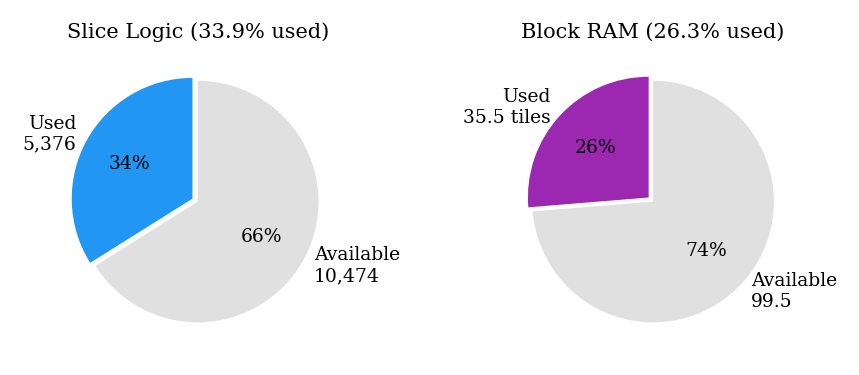
\includegraphics[width=0.85\textwidth]{figures/fig_resource_pie.png}
\caption{FPGA resource utilization for the complete E203 SoC with CNN NICE accelerator (post-placement).}
\label{fig:4_4}
\end{figure}

\begin{figure}[htbp]
\centering
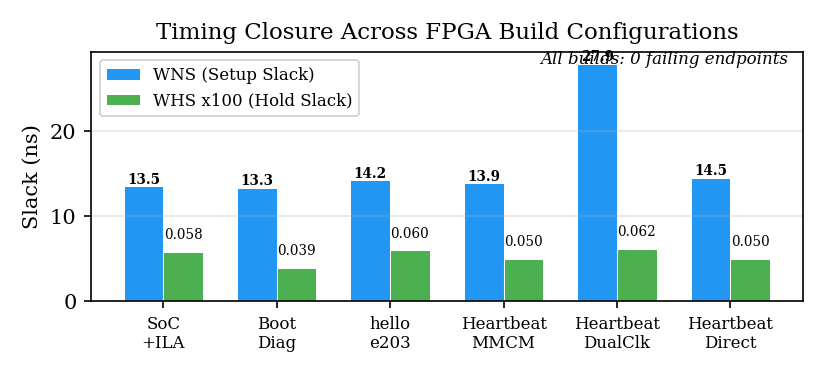
\includegraphics[width=0.85\textwidth]{figures/fig_timing.png}
\caption{Timing closure summary across FPGA build configurations showing all constraints met with positive slack.}
\label{fig:4_5}
\end{figure}

\begin{figure}[htbp]
\centering
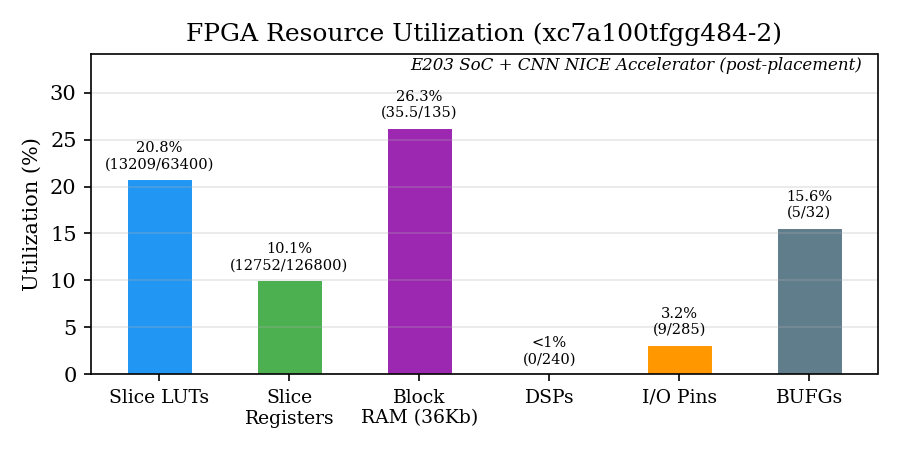
\includegraphics[width=0.85\textwidth]{figures/fig_utilization.png}
\caption{Resource distribution: Slice Logic and Block RAM utilization.}
\label{fig:4_6}
\end{figure}
